%package list
\documentclass{article}
\usepackage[top=3cm, bottom=3cm, outer=3cm, inner=3cm]{geometry}
\usepackage{multicol}
\usepackage{graphicx}
\usepackage{url}
%\usepackage{cite}
\usepackage{hyperref}
\usepackage{array}
%\usepackage{multicol}
\newcolumntype{x}[1]{>{\centering\arraybackslash\hspace{0pt}}p{#1}}
\usepackage{natbib}
\usepackage{pdfpages}
\usepackage{multirow}
\usepackage[normalem]{ulem}
\useunder{\uline}{\ul}{}
\usepackage{svg}
\usepackage{xcolor}
\usepackage{listings}
\lstdefinestyle{ascii-tree}{
    literate={├}{|}1 {─}{--}1 {└}{+}1 
  }
\lstset{basicstyle=\ttfamily,
  showstringspaces=false,
  commentstyle=\color{red},
  keywordstyle=\color{blue}
}
%\usepackage{booktabs}
\usepackage{caption}
\usepackage{subcaption}
\usepackage{float}
\usepackage{array}

\newcolumntype{M}[1]{>{\centering\arraybackslash}m{#1}}
\newcolumntype{N}{@{}m{0pt}@{}}


%%%%%%%%%%%%%%%%%%%%%%%%%%%%%%%%%%%%%%%%%%%%%%%%%%%%%%%%%%%%%%%%%%%%%%%%%%%%
%%%%%%%%%%%%%%%%%%%%%%%%%%%%%%%%%%%%%%%%%%%%%%%%%%%%%%%%%%%%%%%%%%%%%%%%%%%%
\newcommand{\itemEmail}{jperez@unsa.edu.pe}
\newcommand{\itemStudent}{Juan Perez Luna}
\newcommand{\itemCourse}{Programación}
\newcommand{\itemCourseCode}{20231001}
\newcommand{\itemSemester}{I}
\newcommand{\itemUniversity}{Universidad Nacional de San Agustín de Arequipa}
\newcommand{\itemFaculty}{Facultad de Ingeniería de Producción y Servicios}
\newcommand{\itemDepartment}{Departamento Académico de Ingeniería de Sistemas e Informática}
\newcommand{\itemSchool}{Escuela Profesional de Ingeniería de Sistemas}
\newcommand{\itemAcademic}{2023 - A}
\newcommand{\itemInput}{Del 10 Abril 2023}
\newcommand{\itemOutput}{Al 17 Abril 2023}
\newcommand{\itemPracticeNumber}{01}
\newcommand{\itemTheme}{Git y GitHub}
%%%%%%%%%%%%%%%%%%%%%%%%%%%%%%%%%%%%%%%%%%%%%%%%%%%%%%%%%%%%%%%%%%%%%%%%%%%%
%%%%%%%%%%%%%%%%%%%%%%%%%%%%%%%%%%%%%%%%%%%%%%%%%%%%%%%%%%%%%%%%%%%%%%%%%%%%

\usepackage[english,spanish]{babel}
\usepackage[utf8]{inputenc}
\AtBeginDocument{\selectlanguage{spanish}}
\renewcommand{\figurename}{Figura}
\renewcommand{\refname}{Referencias}
\renewcommand{\tablename}{Tabla} %esto no funciona cuando se usa babel
\AtBeginDocument{%
	\renewcommand\tablename{Tabla}
}

\usepackage{fancyhdr}
\pagestyle{fancy}
\fancyhf{}
\setlength{\headheight}{30pt}
\renewcommand{\headrulewidth}{1pt}
\renewcommand{\footrulewidth}{1pt}
\fancyhead[L]{\raisebox{-0.2\height}{
\includegraphics[width=3cm]{img/logo_episunsa.png}}}
\fancyhead[C]{\fontsize{7}{7}\selectfont	\itemUniversity \\ \itemFaculty \\ \itemDepartment \\ \itemSchool \\ \textbf{\itemCourse}}
\fancyhead[R]{\raisebox{-0.2\height}{
\includegraphics[width=1.2cm]{img/logo_abet}}}
\fancyfoot[L]{Estudiante Juan Perez Perez}
\fancyfoot[C]{\itemCourse}
\fancyfoot[R]{Página \thepage}

% para el codigo fuente
\usepackage{listings}
\usepackage{color, colortbl}
\definecolor{dkgreen}{rgb}{0,0.6,0}
\definecolor{gray}{rgb}{0.5,0.5,0.5}
\definecolor{mauve}{rgb}{0.58,0,0.82}
\definecolor{codebackground}{rgb}{0.95, 0.95, 0.92}
\definecolor{tablebackground}{rgb}{0.8, 0, 0}

\lstset{frame=tb,
	language=bash,
	aboveskip=3mm,
	belowskip=3mm,
	showstringspaces=false,
	columns=flexible,
	basicstyle={\small\ttfamily},
	numbers=none,
	numberstyle=\tiny\color{gray},
	keywordstyle=\color{blue},
	commentstyle=\color{dkgreen},
	stringstyle=\color{mauve},
	breaklines=true,
	breakatwhitespace=true,
	tabsize=3,
	backgroundcolor= \color{codebackground},
}

\begin{document}
	
	\vspace*{10px}
	
	\begin{center}	
		\fontsize{17}{17} \textbf{ Informe de Laboratorio \itemPracticeNumber}
	\end{center}
	\centerline{\textbf{\Large Tema: \itemTheme}}
	%\vspace*{0.5cm}	

	\begin{flushright}
		\begin{tabular}{|M{2.5cm}|N|}
			\hline 
			\rowcolor{tablebackground}
			\color{white} \textbf{Nota}  \\
			\hline 
			     \\[30pt]
			\hline 			
		\end{tabular}
	\end{flushright}	

	\begin{table}[H]
		\begin{tabular}{|x{4.7cm}|x{4.8cm}|x{4.8cm}|}
			\hline 
			\rowcolor{tablebackground}
			\color{white} \textbf{Estudiante} & \color{white}\textbf{Escuela}  & \color{white}\textbf{Asignatura}   \\
			\hline 
			{\itemStudent \par \itemEmail} & \itemSchool & {\itemCourse \par Semestre: \itemSemester \par Código: \itemCourseCode}     \\
			\hline 			
		\end{tabular}
	\end{table}		
	
	\begin{table}[H]
		\begin{tabular}{|x{4.7cm}|x{4.8cm}|x{4.8cm}|}
			\hline 
			\rowcolor{tablebackground}
			\color{white}\textbf{Laboratorio} & \color{white}\textbf{Tema}  & \color{white}\textbf{Duración}   \\
			\hline 
			\itemPracticeNumber & \itemTheme & 04 horas   \\
			\hline 
		\end{tabular}
	\end{table}
	
	\begin{table}[H]
		\begin{tabular}{|x{4.7cm}|x{4.8cm}|x{4.8cm}|}
			\hline 
			\rowcolor{tablebackground}
			\color{white}\textbf{Semestre académico} & \color{white}\textbf{Fecha de inicio}  & \color{white}\textbf{Fecha de entrega}   \\
			\hline 
			\itemAcademic & \itemInput &  \itemOutput  \\
			\hline 
		\end{tabular}
	\end{table}
	
	\section{Tipos de Datos:}
	\begin{itemize}		
		\item La página web que diseñamos es útil para la cafetería Caffe.Aqp con una óptima interacción humano-computadora y características centradas en la eficiencia operativa y la satisfacción del cliente tiene el potencial de revolucionar la forma en que las cafeterías gestionan sus operaciones y brindan servicios a sus clientes. La plataforma ofrece una solución integral que beneficia tanto a los administradores como a los clientes, creando una experiencia más conveniente y placentera en todos los aspectos. La página web se ha desarrollado con el propósito de optimizar la gestión de productos, pedidos, reservas de mesas y la generación de boletas.
	\end{itemize}
		
	\section{Requisitos del sistema}
	\begin{itemize}
		\item El sistema debe satisfacer los siguientes requisitos funcionales y no funcionales:
		\item RQ01 : El sistema debe estar disponible en Internet a través de una URL.
		\item RQ02 : El sistema debe permitir el inicio/cierre de sesión.
		\item RQ03 : El sistema debe permitir gestionar los productos ingresados y los eliminados solo a los administradores.
		\item RQ04 : El sistema debe permitir poder configurar cada uno de los atributos de los productos solo a los administradores.
		\item RQ05 : El sistema debe permitir realizar reservaciones para cada uno de los clientes..
		\item RQ06 : El sistema debe permitir realizar compras en línea.
  	\item RQ07: El sistema debe enviar 
        notificaciones por correo electrónico, cuando se realice una compra.
		\item RQ08: El sistema debe ser compatible con dispositivos móviles.
	\end{itemize}
	
	\section{Modelado de datos}
	\begin{itemize}
		\item El modelo de comidas: En esta entidad se guardarán cada uno de los productos ingresados. Los atributos por los que estará compuesto esta entidad son: id, que será su código único, name el cual será el nombre del producto, tipos el cual indicará si es bebida comida o postre, imagen para poder guardar una imagen en el, desc la cual es una breve descripción del producto y por último price que será el precio del producto.
        \begin{lstlisting}[language=bash,caption={Modelado de comidas}][H]
		class comidas(models.Model):
           id = int
           name = models.CharField(max_length=100)
           tipo = models.CharField(max_length=2, choices=Tipo, default='4')
           img = models.ImageField(upload_to='pics')
           desc = models.TextField(default='')
           price = models.IntegerField()

  	\end{lstlisting}
		\item El modelo de  clientes: En esta entidad se guardaran los clientes que ingresamos en nuestra bd. Los atributos que contendrá nuestra entidad son nombre, el cual obtendrá el nombre de este, email, el cual contendrá su email donde se enviará su boleta de compra y por último su teléfono para poder comunicarnos con el.
        \begin{lstlisting}[language=bash,caption={Modelo de clientes}][H]
		
       class Cliente(models.Model):
          nombre = models.CharField(max_length=100)
          email = models.EmailField()
          telefono = models.CharField(max_length=20)

        def __str__(self):
            return self.nombre
    
        class Meta:
            ordering = ['nombre']

        def get_absolute_url(self):
            return reverse('cliente-detail', args=[str(self.id)])
	  \end{lstlisting}
		\item El modelo de Pedido: En esta entidad podremos guardar los valores de los Pedidos realizados, comenzando por el cliente el cual realizó dicho pedido, la fecha en la que se adquirió el pedido y los productos adquiridos, También tendrá un modelo de nombre ESTADOSPEDIDO, para saber si esta pendiente, ya se esta realizando o se completo.
        \begin{lstlisting}[language=bash,caption={Modelo de pedido}][H]
		class Pedido(models.Model):
              cliente = models.ForeignKey('Cliente', on_delete=models.CASCADE)
              fecha = models.DateTimeField(auto_now_add=True)
              productos = models.ManyToManyField('Producto', through='ItemPedido')
            ESTADOS_PEDIDO = [
                ('P', 'Pendiente'),
                ('E', 'En preparación'),
                ('C', 'Completado'),
            ]
             estado = models.CharField(max_length=1, choices=ESTADOS_PEDIDO, default='P')

             def __str__(self):
                 return f"Pedido {self.cliente} - {self.id}"

	  \end{lstlisting}
		\item El modelo ITEMPEDIDO: Esta entidad viene a ser de relación, entre producto y pedido, donde tendrá el llamado de ambas tablas y se le añadirá el valor de cantidad.
        \begin{lstlisting}[language=bash,caption={Modelo ITEMPEDIDO}][H]
	      class ItemPedido(models.Model):
                pedido = models.ForeignKey('Pedido', on_delete=models.CASCADE)
                producto = models.ForeignKey('Producto', on_delete=models.CASCADE)
                cantidad = models.PositiveIntegerField()

                def subtotal(self):
                    return self.cantidad * self.producto.precio

                def __str__(self):
                return f"Pedido {self.producto.nombre}, Cantidad {self.cantidad}, Precio unitario {self.producto.precio}"
	  \end{lstlisting}
        \item El modelo carrito: Esta entidad será de referencia para saber qué productos se adquirió.
        \begin{lstlisting}[language=bash,caption={Modelo de carrio}][H]
		    class Carrito(models.Model):
                cliente = models.OneToOneField('Cliente', on_delete=models.CASCADE)
                productos = models.ManyToManyField('Producto', through='ItemCarrito')

                def __str__(self):
                    return f"Carrito de {self.cliente.nombre}"
	  \end{lstlisting}
        \item El modelo ReservaMesa: Esta entidad sirve para poder guardar la información de las mesas que serán reservadas, se guardará el cliente, la fecha en la que se hará la reserva, la hora en la que se acercara el cliente, y la cantidad de personas que asistiran.
        \begin{lstlisting}[language=bash,caption={Modelo de ReservaMesa}][H]
		     class ReservaMesa(models.Model):
                cliente = models.ForeignKey('Cliente', on_delete=models.CASCADE)
                fecha = models.DateField()
                hora = models.TimeField()
                cantidad_personas = models.PositiveIntegerField()

                def __str__(self):
                    return f"Reserva para {self.cantidad_personas} personas el {self.fecha} a las {self.hora}"
	  \end{lstlisting}
  
	\end{itemize}
	
	\section{Actividades con el repositorio GitHub}
	
	\subsection{Creando e inicializando repositorio GitHub}
	\begin{itemize}	
		\item Como es el primer laboratorio se creo el repositorio GitHub.
		\item Se realizaron los siguientes comandos en la computadora:
	\end{itemize}	
		
	\begin{lstlisting}[language=bash,caption={Creando directorio de trabajo}][H]
		$ mkdir -p $HOME/rescobedoq/
	\end{lstlisting}
	\begin{lstlisting}[language=bash,caption={Dirijíéndonos al directorio de trabajo}][H]
		$ cd $HOME/rescobedoq/
	\end{lstlisting}	
	\begin{lstlisting}[language=bash,caption={Creando directorio para repositorio GitHub}][H]
		$ mkdir -p $HOME/rescobedoq/programacion
	\end{lstlisting}
	\begin{lstlisting}[language=bash,caption={Inicializando directorio para repositorio GitHub}][H]
		$ cd $HOME/rescobedoq/programacion
		$ echo "# programacion" >> README.md
		$ git init
		$ git config --global user.name "Richart Smith Escobedo Quispe"
		$ git config --global user.email rescobedoq@gmail.com
		$ git add README.md
		$ git commit -m "first commit"
		$ git branch -M main
		$ git remote add origin https://github.com/rescobedoq/programacion.git
		$ git push -u origin main
	\end{lstlisting}
	
	\subsection{Commits}
	\begin{lstlisting}[language=bash,caption={Primer Commit Creando carpeta/archivo para laboratorio 01}][H]
		$ mkdir lab01
		$ touch lab01/Insertion.java
		$ git add .
		$ git commit -m "Creando carpeta/archivo para laboratorio 01"			
		$ git push -u origin main
	\end{lstlisting}
	
	\begin{itemize}	
		\item Se creo el archivo \textbf{.gitignore} para no considerar los archivos \textbf{*.class} que son innecesarios hacer seguimiento.
	\end{itemize}
	\begin{lstlisting}[language=bash,caption={Creando .gitignore}][H]
		$ vim lab01/.gitignore
	\end{lstlisting}
	\begin{lstlisting}[language=bash,caption={lab01/.gitignore}][H]
		*.class
	\end{lstlisting}
	\begin{lstlisting}[language=bash,caption={Commit: Creando .gitignore para archivos *.class}][H]
		$ git add .
		$ git commit -m "Creando .gitignore para archivos *.class"			
		$ git push -u origin main
	\end{lstlisting}
	
	\begin{itemize}	
		\item Para el siguiente commit se implemento el algoritmo de ordenamiento por Inserción, se imprime el arreglo caso definido en el mismo código.
		\item El pseudocódigo utilizado es el siguiente:
	\end{itemize}	
	
	\begin{figure}[H]
		\centering
		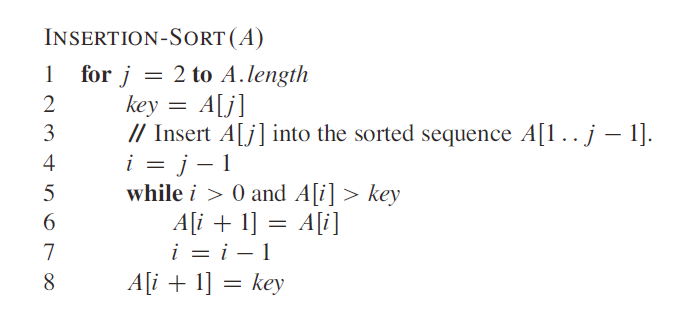
\includegraphics[width=0.8\textwidth,keepaspectratio]{img/pseudocodigo_insercion.png}
		%\includesvg{img/automata.svg}
		%\label{img:mot2}
		%\caption{Product backlog.}
	\end{figure}
	
	\clearpage
	
	\begin{lstlisting}[language=bash,caption={Creando .gitignore}][H]
		$ vim lab01/Insertion.java
	\end{lstlisting}

	
	\begin{lstlisting}[language=bash,caption={Compilando y probando código}][H]
		$ cd lab01
		$ javac Insertion.java
		$ java Insertion
		5 2 4 6 1 3 
		5 5 4 6 1 3 
		2 5 5 6 1 3 
		2 4 5 6 1 3 
		2 2 4 5 6 3 
		1 2 4 4 5 6
	\end{lstlisting}
	\begin{lstlisting}[language=bash,caption={Commit: Probando algoritmo de Inserción con arreglo}][H]
		$ git add .
		$ git commit -m "Probando algoritmo de Insercion con arreglo"			
		$ git push -u origin main
	\end{lstlisting}
	
		
	\subsection{Estructura de laboratorio 01}
	\begin{itemize}	
		\item El contenido que se entrega en este laboratorio es el siguiente:
	\end{itemize}
	
\begin{lstlisting}[style=ascii-tree]
lab01/
|--- Insertion.java
|--- latex
    |--- img
    |   |--- logo_abet.png
    |   |--- logo_episunsa.png
    |   |--- logo_unsa.jpg
    |   |--- pseudocodigo_insercion.png    
    |--- programacion_lab01_rescobedoq_v1.0.pdf    
    |--- programacion_lab01_rescobedoq_v1.0.tex
    |--- src
        |--- Insertion01.java
\end{lstlisting}    

\section{Pregunta: ¿Cúal es el comportamiento del algoritmo de ordenamiento por inserción?}
	\begin{itemize}
		\item El algoritmo muestra un comportamiento cuadrático de O(n²).
		\item Se trabajarón los peores casos desde una arreglo de tamaño 1 hasta N.
		\item Para obtener un grafico ideal se utilizó N=10,000.
	\end{itemize}		

	\section{\textcolor{red}{Rúbricas}}
	
	\subsection{\textcolor{red}{Entregable Informe}}
	\begin{table}[H]
		\caption{Tipo de Informe}
		\setlength{\tabcolsep}{0.5em} % for the horizontal padding
		{\renewcommand{\arraystretch}{1.5}% for the vertical padding
		\begin{tabular}{|p{3cm}|p{12cm}|}
			\hline
			\multicolumn{2}{|c|}{\textbf{\textcolor{red}{Informe}}}  \\
			\hline 
			\textbf{\textcolor{red}{Latex}} & \textcolor{blue}{El informe está en formato PDF desde Latex,  con un formato limpio (buena presentación) y facil de leer.}   \\ 
			\hline 
			
			
		\end{tabular}
	}
	\end{table}
	
	\clearpage
	
	\subsection{\textcolor{red}{Rúbrica para el contenido del Informe y demostración}}
	\begin{itemize}			
		\item El alumno debe marcar o dejar en blanco en celdas de la columna \textbf{Checklist} si cumplio con el ítem correspondiente.
		\item Si un alumno supera la fecha de entrega,  su calificación será sobre la nota mínima aprobada, siempre y cuando cumpla con todos lo items.
		\item El alumno debe autocalificarse en la columna \textbf{Estudiante} de acuerdo a la siguiente tabla:
	
		\begin{table}[ht]
			\caption{Niveles de desempeño}
			\begin{center}
			\begin{tabular}{ccccc}
    			\hline
    			 & \multicolumn{4}{c}{Nivel}\\
    			\cline{1-5}
    			\textbf{Puntos} & Insatisfactorio 25\%& En Proceso 50\% & Satisfactorio 75\% & Sobresaliente 100\%\\
    			\textbf{2.0}&0.5&1.0&1.5&2.0\\
    			\textbf{4.0}&1.0&2.0&3.0&4.0\\
    		\hline
			\end{tabular}
		\end{center}
	\end{table}	
	
	\end{itemize}
	
	\begin{table}[H]
		\caption{Rúbrica para contenido del Informe y demostración}
		\setlength{\tabcolsep}{0.5em} % for the horizontal padding
		{\renewcommand{\arraystretch}{1.5}% for the vertical padding
		%\begin{center}
		\begin{tabular}{|p{2.7cm}|p{7cm}|x{1.3cm}|p{1.2cm}|p{1.5cm}|p{1.1cm}|}
			\hline
    		\multicolumn{2}{|c|}{Contenido y demostración} & Puntos & Checklist & Estudiante & Profesor\\
			\hline
			\textbf{1. GitHub} & Hay enlace URL activo del directorio para el  laboratorio hacia su repositorio GitHub con código fuente terminado y fácil de revisar. &2 &X &2 & \\ 
			\hline
			\textbf{2. Commits} &  Hay capturas de pantalla de los commits más importantes con sus explicaciones detalladas. (El profesor puede preguntar para refrendar calificación). &4 & & & \\ 
			\hline 
			\textbf{3. Código fuente} &  Hay porciones de código fuente importantes con numeración y explicaciones detalladas de sus funciones. &2 &X &2 & \\ 
			\hline 
			\textbf{4. Ejecución} & Se incluyen ejecuciones/pruebas del código fuente  explicadas gradualmente. &2 &X &2 & \\ 
			\hline			
			\textbf{5. Pregunta} & Se responde con completitud a la pregunta formulada en la tarea.  (El profesor puede preguntar para refrendar calificación).  &2 &X &2 & \\ 
			\hline	
			\textbf{6. Fechas} & Las fechas de modificación del código fuente estan dentro de los plazos de fecha de entrega establecidos. &2 &X &2 & \\ 
			\hline 
			\textbf{7. Ortografía} & El documento no muestra errores ortográficos. &2 &X &2 & \\ 
			\hline 
			\textbf{8. Madurez} & El Informe muestra de manera general una evolución de la madurez del código fuente,  explicaciones puntuales pero precisas y un acabado impecable.   (El profesor puede preguntar para refrendar calificación).  &4 & & & \\ 
			\hline
			\multicolumn{2}{|c|}{\textbf{Total}} &20 & &12 & \\ 
			\hline
		\end{tabular}
		%\end{center}
		%\label{tab:multicol}
		}
	\end{table}
	
\clearpage

\section{Referencias}
\begin{itemize}			
	\item \url{https://www.w3schools.com/java/default.asp}
	\item \url{https://www.geeksforgeeks.org/insertion-sort/}
\end{itemize}	
	
%\clearpage
%\bibliographystyle{apalike}
%\bibliographystyle{IEEEtranN}
%\bibliography{bibliography}
			
\end{document}